% Options for packages loaded elsewhere
\PassOptionsToPackage{unicode}{hyperref}
\PassOptionsToPackage{hyphens}{url}
%
\documentclass[
]{article}
\usepackage{amsmath,amssymb}
\usepackage{lmodern}
\usepackage{iftex}
\ifPDFTeX
  \usepackage[T1]{fontenc}
  \usepackage[utf8]{inputenc}
  \usepackage{textcomp} % provide euro and other symbols
\else % if luatex or xetex
  \usepackage{unicode-math}
  \defaultfontfeatures{Scale=MatchLowercase}
  \defaultfontfeatures[\rmfamily]{Ligatures=TeX,Scale=1}
  \setmainfont[]{SourceSansPro}
\fi
% Use upquote if available, for straight quotes in verbatim environments
\IfFileExists{upquote.sty}{\usepackage{upquote}}{}
\IfFileExists{microtype.sty}{% use microtype if available
  \usepackage[]{microtype}
  \UseMicrotypeSet[protrusion]{basicmath} % disable protrusion for tt fonts
}{}
\makeatletter
\@ifundefined{KOMAClassName}{% if non-KOMA class
  \IfFileExists{parskip.sty}{%
    \usepackage{parskip}
  }{% else
    \setlength{\parindent}{0pt}
    \setlength{\parskip}{6pt plus 2pt minus 1pt}}
}{% if KOMA class
  \KOMAoptions{parskip=half}}
\makeatother
\usepackage{xcolor}
\usepackage[margin=1in]{geometry}
\usepackage{graphicx}
\makeatletter
\def\maxwidth{\ifdim\Gin@nat@width>\linewidth\linewidth\else\Gin@nat@width\fi}
\def\maxheight{\ifdim\Gin@nat@height>\textheight\textheight\else\Gin@nat@height\fi}
\makeatother
% Scale images if necessary, so that they will not overflow the page
% margins by default, and it is still possible to overwrite the defaults
% using explicit options in \includegraphics[width, height, ...]{}
\setkeys{Gin}{width=\maxwidth,height=\maxheight,keepaspectratio}
% Set default figure placement to htbp
\makeatletter
\def\fps@figure{htbp}
\makeatother
\setlength{\emergencystretch}{3em} % prevent overfull lines
\providecommand{\tightlist}{%
  \setlength{\itemsep}{0pt}\setlength{\parskip}{0pt}}
\setcounter{secnumdepth}{-\maxdimen} % remove section numbering
\usepackage[default]{sourcesanspro}
\usepackage[T1]{fontenc}
\ifLuaTeX
  \usepackage{selnolig}  % disable illegal ligatures
\fi
\IfFileExists{bookmark.sty}{\usepackage{bookmark}}{\usepackage{hyperref}}
\IfFileExists{xurl.sty}{\usepackage{xurl}}{} % add URL line breaks if available
\urlstyle{same} % disable monospaced font for URLs
\hypersetup{
  pdftitle={Session 1 : Summary of the data set},
  pdfauthor={Moonbin Jo},
  hidelinks,
  pdfcreator={LaTeX via pandoc}}

\title{Session 1 : Summary of the data set}
\author{Moonbin Jo}
\date{}

\begin{document}
\maketitle

\hypertarget{section}{%
\section{}\label{section}}

\hypertarget{objectives-of-this-session}{%
\subsection{Objectives of this
session}\label{objectives-of-this-session}}

\begin{itemize}
\tightlist
\item
  Understanding the data set of perception
\item
  Analysis and visualization of data

  \begin{itemize}
  \tightlist
  \item
    Yes/No answer data
  \item
    Score data
  \end{itemize}
\end{itemize}

\hypertarget{exercises}{%
\subsection{Exercises}\label{exercises}}

\hypertarget{introduction-of-data-set}{%
\subsubsection{Introduction of data
set}\label{introduction-of-data-set}}

This data set is a part of an experimental project on the power of
habits on climate change, as well as people's personal capacity to
implement them in their everyday lives.

The participants were provided with a list of ten habits that could
implement in their daily lives.

The study is trying to persuade participants into implementing these
habits in their everyday lives. However, persuading participants into
implementing particular habits is not possible without an understanding
of the perception of habits. Some habits are more difficult than others,
and if we try to persuade participants into implementing habits that are
perceived as too difficult, the participants will think it is not
possible.

By understanding the difficulty and constraint of implementation, and
the reasons why the habits are perceived that way, we can have a deeper
understanding in the perception of the habits. This will help us in
persuading the participants to implement the habits.

The questionnaire regarding the perception of the ten habits was
composed of three sections.

The first section of the questionnaire was about the possibility of
implementation of the habit. If the participant thought the habit as
implementable in the near future, or if they had already started, they
would answer ``Yes''. If they found the habit as not possible to
implement in the near future, they would answer ``No''.

The second section of the questionnaire asked the participants about the
amount of constraint the participants would experience from implementing
the habit. This was answered with a scale from 0 to 5.

The third section asked the reasons on their answers, and would give us
a more thorough explanation on their answers, giving us more insight on
the perception of difficulty of these habits.

In this session, we will look into analysis and visualization of the
first and second section of the questionnaire. We will try and deepen
our understanding in the implementation and constraint of the ten
habits.

\hypertarget{analysis-and-visualization-of-data}{%
\subsubsection{Analysis and visualization of
data}\label{analysis-and-visualization-of-data}}

\hypertarget{yesno-answer-data}{%
\paragraph{Yes/No answer data}\label{yesno-answer-data}}

\hypertarget{analysis}{%
\subparagraph{Analysis}\label{analysis}}

The first section of the data is made up of answers of Yes or No.~So
what can we do with this data? We can first understand the difficulty in
implementation by investigating the frequency of answers.

If you want additional information about what categorical variables are,
please visit
\href{https://www150.statcan.gc.ca/n1/edu/power-pouvoir/ch8/5214817-eng.htm}{this
website}.

\begin{verbatim}
##  car_alone never_airplane loaner    clothes_second  bulk     local_products
##  Yes:79    Yes:81         Yes:151   Yes:95         Yes:118   Yes:89        
##  No :88    No :86         No : 16   No :72         No : 49   No :78        
##  unplug    low_temperature vegetarian air_drying
##  Yes:144   Yes:145         Yes: 39    Yes:154   
##  No : 23   No : 22         No :128    No : 13
\end{verbatim}

Looking at these results, we can see that the proportion of answers are
different from each other. If the proportion of ``No'' is higher, more
people find this habit to be more difficult to implement. Therefore, if
we organize the order of these habits regarding the proportion of the
answer ``No'', we can see which habits are harder to implement than
others.

\begin{verbatim}
##                 Yes  No
## vegetarian       39 128
## car_alone        79  88
## never_airplane   81  86
## local_products   89  78
## clothes_second   95  72
## bulk            118  49
## unplug          144  23
## low_temperature 145  22
## loaner          151  16
## air_drying      154  13
\end{verbatim}

By rearranging the habits regarding the frequencies in answers, we can
see that the habits of becoming vegetarian and never using one's car
when they are alone are the hardest to implement. We can also see that
air drying your laundry and using a loaner system for items are easier
to implement.

\hypertarget{visualization-of-the-yesno-data}{%
\subparagraph{Visualization of the Yes/No
data}\label{visualization-of-the-yesno-data}}

Though we could stop and call it a day on the analysis of the Yes/No
data, the results are still a list of numbers and letters that we have
to take time to interpret. A more effective way of presenting the data
is by visualizing it. This will be done by using the \texttt{ggplot2}
package.

\hypertarget{what-are-packages}{%
\subparagraph{What are packages?}\label{what-are-packages}}

R by default has a number of functions you can use, but you can utilize
a wider range of functions by using packages. R packages are collections
of R functions, code and data that can be installed and utilized easily.
When R is first opened, the R console only has the default packages. But
by loading other packages using the function \texttt{library()}, we have
access to more functions.

The data we have put together is the frequency of the answers by each
habit. This sort of data can be visualized using bar plots. First let's
visualize the habit that was considered most easy to implement.

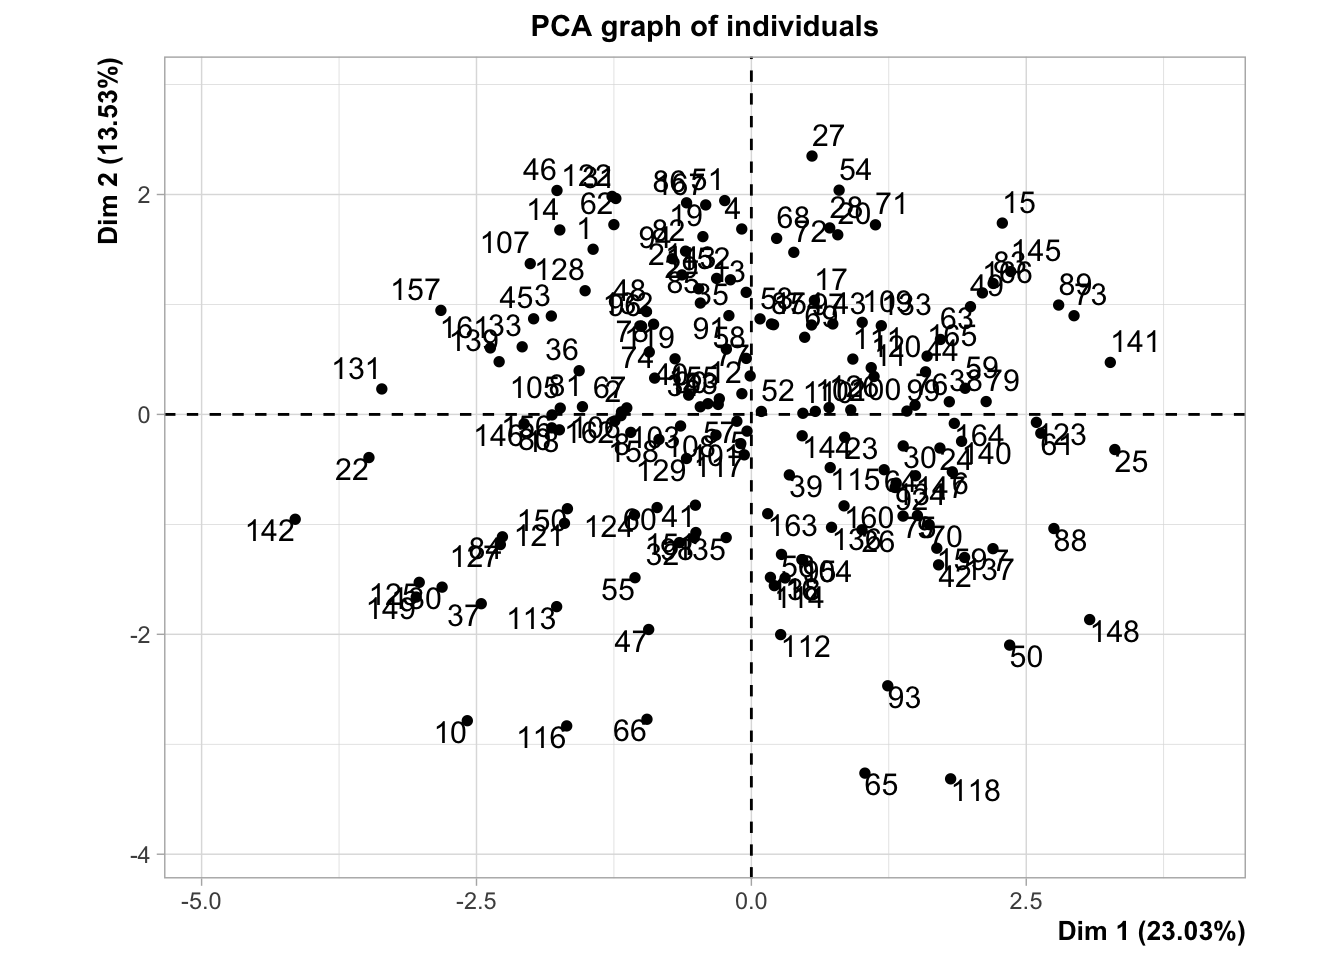
\includegraphics{S1_files/figure-latex/unnamed-chunk-4-1.pdf}

Through this bar plot we can see that the frequency of the answer
``Yes'' is much higher than ``No''.

We can see that the frequency of the answer ``Yes'' is much higher than
``No'', meaning that the habit of air drying your laundry is found
implementable for a lot of people. Now let's look at the habit that was
considered most difficult to implement.

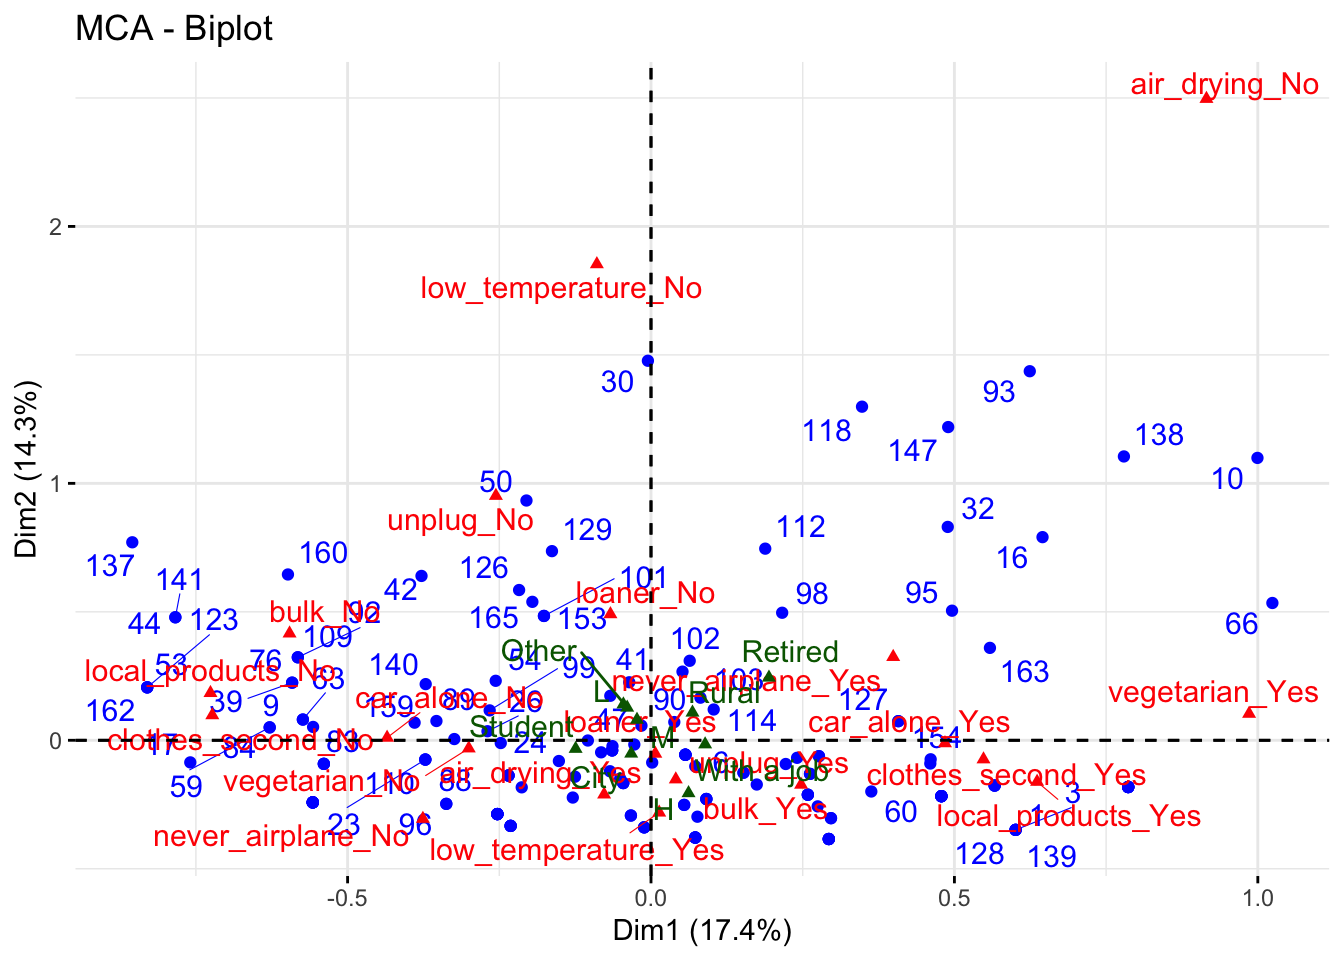
\includegraphics{S1_files/figure-latex/unnamed-chunk-5-1.pdf}

Unlike the previous habit, the habit of becoming vegetarian had a higher
frequency of the answer ``No''. This shows that the implementation of
this habit is difficult to implement.

In order to effectively compare the proportions of these two habits, we
can standardize the y axis and put these graphs side by side.

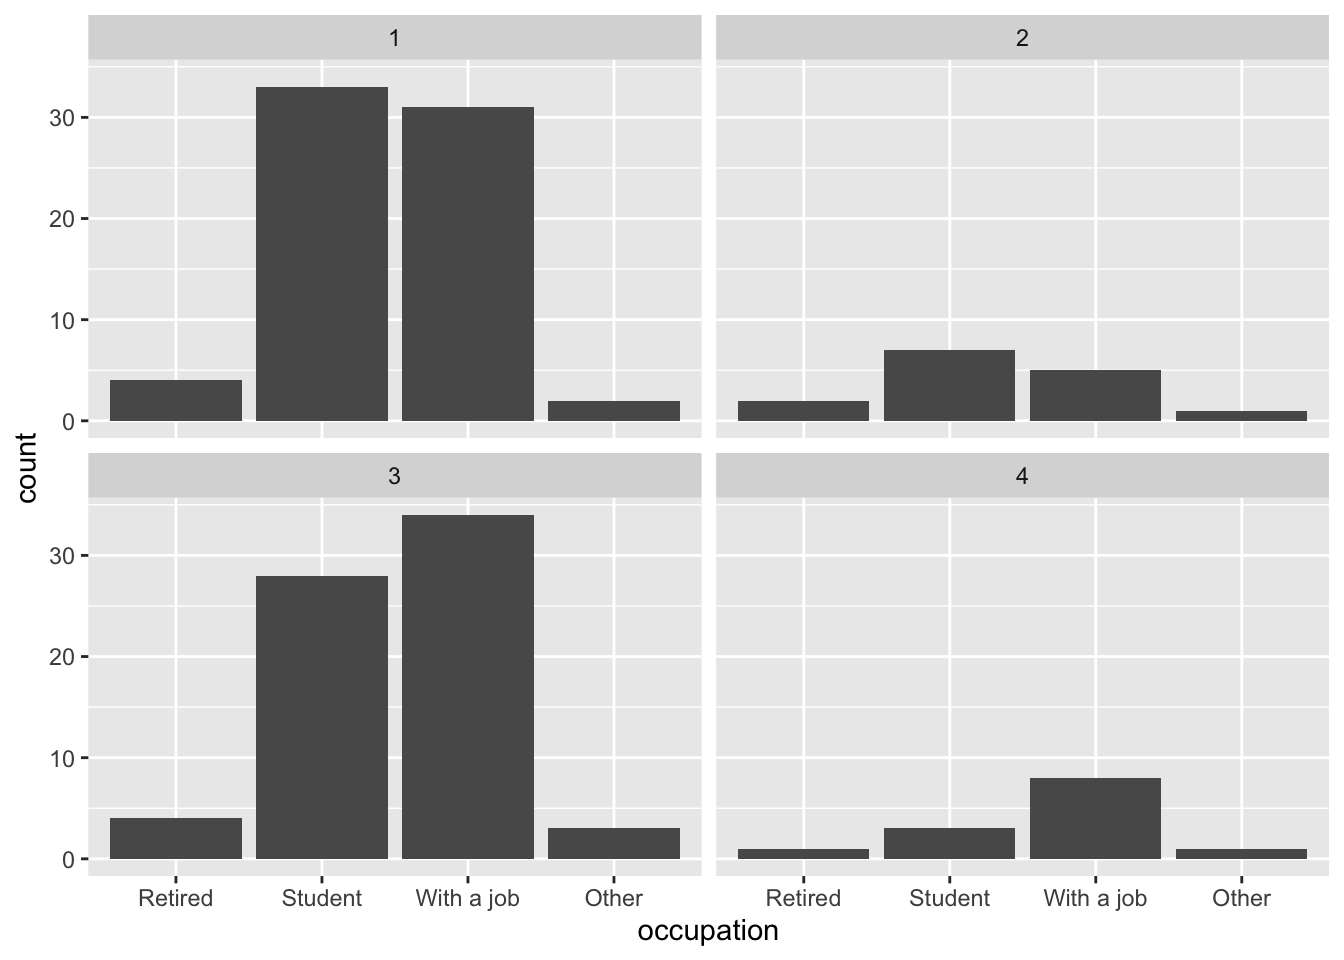
\includegraphics{S1_files/figure-latex/unnamed-chunk-6-1.pdf}

Through this comparison, we can see that the difference in proportions
is more extreme for the habit of air drying than becoming vegetarian.
Through these bar plots have visualized the proportions of the answers
in a way where we don't have to read any numbers, and therefore, we can
call it a day for this data.

\hypertarget{score-data}{%
\paragraph{Score data}\label{score-data}}

\hypertarget{data-analysis-of-the-score-data}{%
\subparagraph{Data analysis of the score
data}\label{data-analysis-of-the-score-data}}

The second section of the data is about the score of constraint for the
ten habits. With this data, we can understand the quantitative amount of
constraint the participants perceive for the ten habits. A rudimentary
analysis can be achieved by calculating the mean values of scores for
each habit. We'll first look at this.

\begin{verbatim}
##       car_alone_score  never_airplane_score          loaner_score 
##                   3.1                   2.7                   1.7 
##  clothes_second_score            bulk_score  local_products_score 
##                   2.3                   2.4                   2.7 
##          unplug_score low_temperature_score      vegetarian_score 
##                   1.6                   1.5                   3.6 
##      air_drying_score 
##                   1.1
\end{verbatim}

By looking at the mean values of the scores, we can see that the habits
have different mean values, showing that the amount of constraint
participants perceive of the habit is different. Just like the Yes/No
data, we can rearrange the data to understand the data more. In this
section, we can use the mean values of score can be used to order the
habits.

\begin{verbatim}
##      vegetarian_score       car_alone_score  never_airplane_score 
##                   3.6                   3.1                   2.7 
##  local_products_score            bulk_score  clothes_second_score 
##                   2.7                   2.4                   2.3 
##          loaner_score          unplug_score low_temperature_score 
##                   1.7                   1.6                   1.5 
##      air_drying_score 
##                   1.1
\end{verbatim}

By rearranging habits by mean values we can see which habits are more
constraining than others. We can also see that out of the habits,
becoming vegetarian is the most constraining, while air drying is the
least constraining.

\hypertarget{visualization-of-the-score-data}{%
\subparagraph{Visualization of the score
data}\label{visualization-of-the-score-data}}

The mean value of the scores shows a good summary of the amount of
constraint, but it does not explain the data we have fully. Even if two
habits have similar mean values, it does not mean that the distribution
of perception is the same. Some habits may have a rather equal
proportion in scores, meaning that some participants found this habit to
be easy and others found this habit to be hard. On the other hand, some
habits may have skewed distribution, meaning that the difficulty in the
habit is similar for the participants. The score's distribution will be
visualized with a histogram. This will show the frequency of score
answers for each habit.

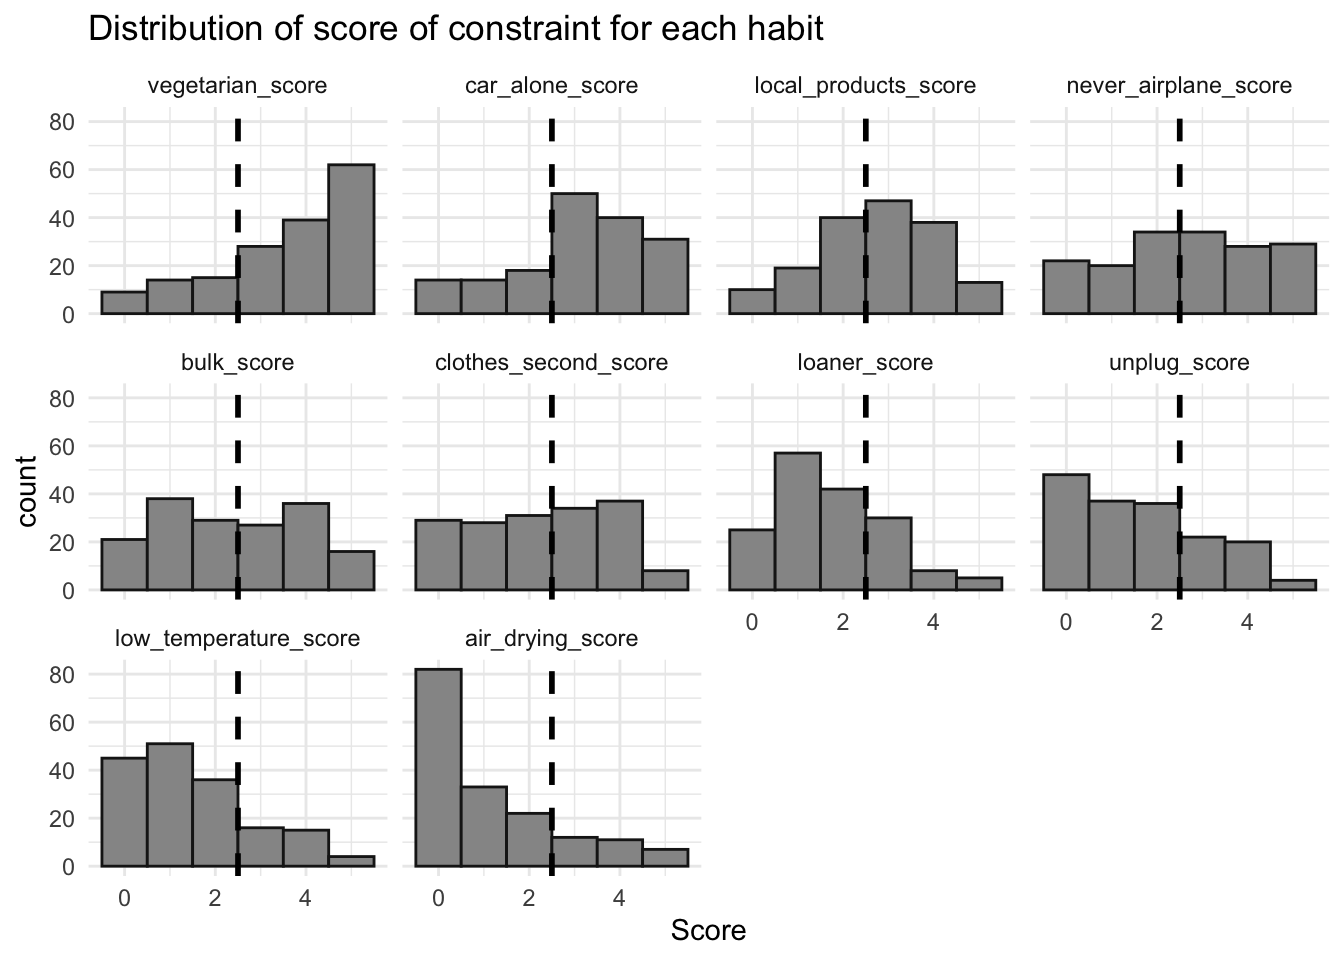
\includegraphics{S1_files/figure-latex/unnamed-chunk-9-1.pdf}

Now we can see the distribution of scores, we can have a deeper
understanding in the scores. For example, the habit of only using local
products (\texttt{local\_products\_score}) and never taking an airplane
(\texttt{never\_airplane\_score}) have the same mean value of 2.7, but
they have a difference in distribution.

For the habit of using local products, the score answers were more
heavily distributed between the scores of 2-4, indicating that the
majority participants perceived this habit to have a similar amount of
constraint. However, for the habit of never flying on an airplane, the
distribution was rather even, indicating that for some participants this
habit was perceived as not constraining at all, while for others it was
very constraining.

Through this session we have analyzed categorical data and continuous
data, and also presented this analysis in a more effective way by
visualizing the data. In the next session, we will look deeper into the
score data in order to deepen our understanding in it.

\hypertarget{vocabulary-of-this-session}{%
\subsection{Vocabulary of this
session}\label{vocabulary-of-this-session}}

\hypertarget{r-commands}{%
\subsubsection{R commands}\label{r-commands}}

\begin{itemize}
\tightlist
\item
  library
\item
  geom\_bar
\item
  geom\_histogram
\end{itemize}

\hypertarget{r-environment}{%
\subsubsection{R environment}\label{r-environment}}

\begin{itemize}
\tightlist
\item
  packages
\end{itemize}

\hypertarget{statistical-terms}{%
\subsubsection{Statistical terms}\label{statistical-terms}}

\begin{itemize}
\tightlist
\item
  Counting frequencies
\item
  Calculating the mean value
\end{itemize}

\end{document}
